\RussianSourceFrame{GELFAND-P001445}{30}
Построим комплекс по этим данным
\begin{equation*}
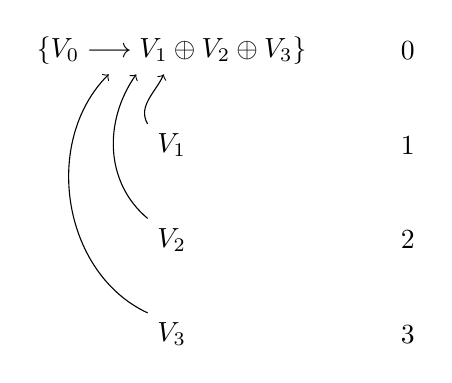
\begin{tikzpicture}
\node (c) at (0,0) {$\{V_0\longrightarrow V_1\oplus V_2\oplus V_3\}$};
\node (v1) at (0,-1.2) {$V_1$};
\node (v2) at (0,-2.4) {$V_2$};
\node (v3) at (0,-3.6) {$V_3$};
\node at (3,0) {$0$};
\node at (3,-1.2) {$1$};
\node at (3,-2.4) {$2$};
\node at (3,-3.6) {$3$};
\draw[->] (v1.north west) to[out=120,in=245] (-0.1,-0.3);
\draw[->] (v2.north west) to[out=140,in=235] (-0.45,-0.3);
\draw[->] (v3.north west) to[out=155,in=225] (-0.8,-0.3);
\end{tikzpicture}
\end{equation*}
Это объект производной категории (предст. колчана)
\begin{equation*}
\begin{tikzcd}[column sep=large,row sep=small]
 & 1 \arrow[dl]\\
0 & 2 \arrow[l]\\
 & 3 \arrow[ul]
\end{tikzcd}
\end{equation*}
Факторизации в обычной кат. надо сопоставлять само
отображение (комплекс)

\RussianUnclear{GELFAND-P001445}{bottom-name}{Парти… [фамилия неразборчива]} ставит и решает вопрос о том, когда производная
катег. совп. с этой (для $3^{\text{х}}$, но не для $4^{\text{х}}$).



\RussianSourceFrame{GELFAND-P001446}{unlabelled}
\underline{23. III. 88 г.}\qquad \underline{Сем. Гельфанда.}

\underline{Зелевинский А.}\qquad
\underline{Матроиды и теорема Холла}

\underline{И.М.Г.}

Матроид. [Над следующим словом зачёркнуто: \RussianUnclear{GELFAND-P001446}{intro-deletion}{неразборчивые зачёркнутые знаки}.]
\underline{Пример:} линейно независ. системы векторов.
\begin{equation*}
M_1,M_2\text{ — мн-ва},\qquad \varphi\subset M_1\times M_2
\end{equation*}
(отношение)

Пусть на $M_1$ есть структ. матроида.

Как ввести структ. матроида на $M_2$?
\begin{equation*}
A\subset M_2,\qquad \pi_1\bigl(\pi_2^{-1}(A)\cap\varphi\bigr)
\text{ — мн-во}.
\end{equation*}
[Под тире зачёркнуто: \RussianUnclear{GELFAND-P001446}{image-set-deletion}{неразборчиво}.]

Ранг мн-ва $A$ определяется

$1^{\circ}$. \underline{Теор. Радо}
\begin{equation*}
r_{M_2}(A)=\min_{B\subset A}
\bigl(r_{M_1}(\varphi(B))+|A-B|\bigr),\qquad A\subset M_2.
\end{equation*}

$2^{\circ}$. \underline{Теор. Холла} $\equiv$
[Над фамилией вставлено: \RussianUnclear{GELFAND-P001446}{hall-insertion}{Ф. / $\varphi$}.]

[Зачёркнуто слева: \RussianUnclear{GELFAND-P001446}{hall-left-deletion}{неразборчиво}.]
\underline{Зад. о выборе невест}:
[Над строкой вставлено: мн-во $M$ женихов,
$\operatorname{Card}M\geq\operatorname{Card}N$.]

Если [над $N$ вписано: мн-во] $N$ невест и
[зачёркнуто: $M\geq N$ женихов], каждому жениху $m\in M$
нравятся невесты $A(m)\subset N$; причем
[зачёркнуто: $\forall A\subset N$] $\forall$ подмн-ва
$K\subset N$,
[над формулой зачёркнуто: \RussianUnclear{GELFAND-P001446}{card-deletion}{неразборчивый знак}.]
\begin{equation*}
\operatorname{Card}\left(\bigcup_{n\in K}B(n)\right)
\geq \operatorname{Card}K.
\end{equation*}



\RussianSourceFrame{GELFAND-P001447}{37}
(Здесь $B(n)\subset M$;
[под $B(n)$ через знак равенства:]
мн-во женихов, к-рым нравится $n$, т.е.
\begin{equation*}
B(n)=
\{m:\ n\in A(m)\}
\end{equation*}
[После $=$ зачёркнуто: \RussianUnclear{GELFAND-P001447}{top-b-deletion}{неразборчивый знак}.])

Тогда $\exists$ вз.-однозн. выбор
[зачёркнуто: \RussianUnclear{GELFAND-P001447}{choice-deletion}{неразборчиво}]:
отображение $f:N\longrightarrow M$, для к-рого
\begin{equation*}
f(n)\subset B(n)\qquad \forall n.
\end{equation*}
\RussianUnclear{GELFAND-P001447}{hall-membership}{В источнике: $f(n)\subset B(n)$.}

[Зачёркнута строка: Теор. Холла\quad $\varphi$ — отношение.]

[Зачёркнуто: Теор.]
Сущ. док-во, содержащее алгоритм.

\underline{Сведение к теор. Радо}: в $N$ надо объявить все мн-ва независимыми.

$2^{\circ}\Rightarrow 3^{\circ}$. \underline{Теор. Биркгофа.}

Из теор. Холла следует, что если есть подгруппа $H\subset G$
[под $G$: кон. группа],
то $\exists$ система общих представителей левых и правых
смежных классов.

\underline{И.М.Г.} Есть неск. знаменитых задач, про к-рые всем очевидна
их бессмысленность.

\underline{Пример.} 1) \underline{Аксиома о параллельности}

(почему именно она?)

[Под этой строкой:] \RussianUnclear{GELFAND-P001447}{parallelism-note}{занимались ими / занимались ними}

[Справа от первых двух строк, за вертикальной чертой:]
$\Rightarrow$ неевкл. геом.

2) \underline{Трисекция угла} и квадратура круга.
\begin{equation*}
\text{Трисекция угла}\ \Downarrow\ \text{теор. Галуа}
\end{equation*}

3) \underline{Теор. Ферма}
\begin{equation*}
\Downarrow
\end{equation*}
теор. [зачёркнуто: \RussianUnclear{GELFAND-P001447}{ideals-deletion}{неразборчивая буква}] идеалов (Куммер)
и алгебр. геометрия.
[Справа, за вертикальной чертой:] раб. Фалтингса.

4) \underline{Задача о $4^{\text{х}}$ красках}
\begin{equation*}
\Downarrow\quad ?
\end{equation*}
Стоит разобрать эти работы.

5) \underline{Гипотеза Римана}



\RussianSourceFrame{GELFAND-P001448}{unlabelled}
\underline{А. Рудаков.}\quad
\underline{Векторные расслоения, группы кос и диофантовы уравнения.}

$1^{\circ}$. На $\mathbb{P}^{2}\ (= \mathbb{C}\mathbb{P}^{2})$

рассм. вект. расслоения (или ког. пучки)
\begin{equation*}
E_1,\ E_2,\ E_3 \tag{1}
\end{equation*}
[После $E_1$ зачёркнуто: \RussianUnclear{GELFAND-P001448}{triple-deletion}{неразборчивые знаки}.]
\begin{equation*}
\begin{gathered}
\operatorname{Ext}^{k}(E_j,E_i)=0,\quad j>i,\quad k=0,1,2,\\
\operatorname{Ext}^{k}(E_i,E_i)=
\begin{cases}
0,& k>0,\\
\mathbb{C},& k=0.
\end{cases}
\end{gathered}
\tag{2}
\end{equation*}
[Перед $k=0,1,2$ зачёркнуто: \RussianUnclear{GELFAND-P001448}{ext-deletion}{неразборчивый знак}.]

Такие существуют и если $\dim E_j=x_j$, то
\begin{equation*}
x_1^2+x_2^2+x_3^2=3x_1x_2x_3
\qquad\text{(ур-е Маркова)} \tag{3}
\end{equation*}
(и все [сверху вставлено: целочисл.] решения так реализуются!)

На наборах [сверху вставлено: (1) (их счётное мн-во)]
действ. группа кос и все наборы (1)
сост. 1 орбиту!

$2^{\circ}$.
\begin{equation*}
Q=\mathbb{P}^{1}\times\mathbb{P}^{1}.
\end{equation*}
[После $Q=$ зачёркнуто: \RussianUnclear{GELFAND-P001448}{quadric-deletion}{неразборчивый знак}.]

Тогда берём 4 расслоения $E_1,E_2,E_3,E_4$
с теми же условиями (2); тоже действ. группа кос.

Вместо (3) возникает система диофантовых ур-й
(но соответствие в одну сторону; не доказано, что все реш. получаются).
Это что-то вроде системы корней, где вместо
гр. Вейля возникает группа кос.

$3^{\circ}$. На $\mathbb{P}^{n}$ можно рассм. расслоения
\begin{equation*}
E_1,E_2,\ldots,E_{n+1}\qquad\text{с усл. (2)}
\end{equation*}
и тоже возникает действие группы кос.

\underline{М. Капранов}: о действии группы кос.

\underline{И.М.Г.}

Разрешимые и неразрешимые классификационные задачи.

Нет парам. $\Rightarrow$ классифицируются (ручные)

1 парам $\Rightarrow$
[зачёркнуто: \RussianUnclear{GELFAND-P001448}{classification-correction}{ручные (…)}; над строкой вставлено: полуручные] (tame)

$\geq 2$ парам. $\Rightarrow$ неразреш.
(напр., пары матриц)

и классиф. отн.
[зачёркнуто: \RussianUnclear{GELFAND-P001448}{bottom-deletion}{неразборчиво}]
\begin{equation*}
(A,B)\mapsto(C^{-1}AC,C^{-1}BC).
\end{equation*}



\RussianSourceFrame{GELFAND-P001449}{38}
В неразреш. задачах всегда есть разрешимая часть
(открытая орбита!)

[Над инициалами зачёркнуто: \RussianUnclear{GELFAND-P001449}{top-deletion}{Еф / неразборчиво}.]

\underline{М.К.}
\begin{equation*}
\operatorname{Ext}^{1}(E,E)=0\ \Rightarrow\ \text{жёсткость}
\end{equation*}
(и рассл. такие не имеют параметров)

[Над следующей строкой зачёркнуто: \RussianUnclear{GELFAND-P001449}{sequence-deletion}{Пару / неразборчиво}.]
\begin{equation*}
0\longrightarrow R\longrightarrow E\otimes\operatorname{Hom}(E,F)
\longrightarrow F
\end{equation*}

Пару $(E,F)$ назовём исключительной, если
$\operatorname{Ext}^{j}(F,E)=0$.

Тогда пара $(F,R)$ тоже исключительна.

Получ. действие $\mathbb{Z}$ на таких парах;
выполняются соотношения, дающие косы.

\underline{И.М.Г.} Работа Берншт.-Гельф.-Пономарев:
в предст. графов действ. гр. Кокстера.

Что нужно для занятий, напр., спектр. теорией из общего образ.

1) Предст. графов (4-ка подпр-в и т.п.)

2) Произв. категория.

\underline{Бейлинсон А.}\qquad \underline{Извращенные пучки.}

\underline{И.М.Г.} (о Макферсоне)

\RussianSourceFigure{GELFAND-P001449}{circle-diagram}{Круг с внутренним криволинейным треугольником и несколькими дугами между точками окружности; справа нижняя вершина и соседние дуги удвоены. Сопоставить точные соединения с оригиналом.}

\par\medskip\noindent
\begin{minipage}[c]{0.48\linewidth}\centering
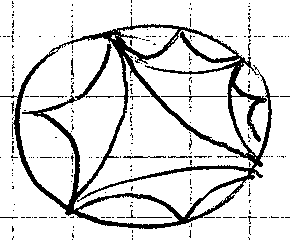
\includegraphics[width=\linewidth]{figures/gelfand-p001449-circle-diagram-original.png}
\par\smallskip{\footnotesize Оригинал рукописного рисунка: GELFAND-P001449\par}
\end{minipage}\hfill
\begin{minipage}[c]{0.48\linewidth}\centering
\resizebox{\linewidth}{!}{% Partial stroke comparison: nearby right-hand endings are not identified as one vertex.
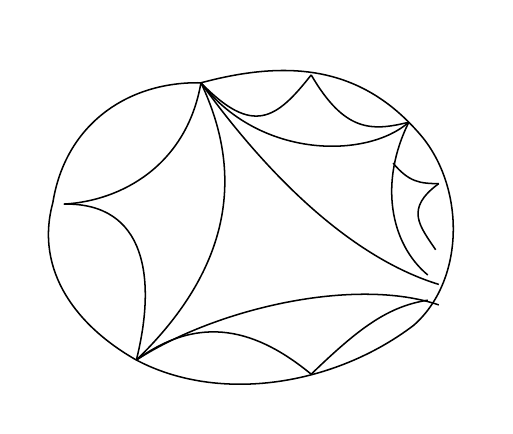
\begin{tikzpicture}[x=0.02cm,y=-0.02cm,line width=0.55pt]
\path[use as bounding box] (0,0) rectangle (290,240);
\draw (110,35)..controls(64,34)and(24,61)..(16,111)
 ..controls(4,155)and(32,190)..(69,211)
 ..controls(122,239)and(195,227)..(245,189)
 ..controls(277,161)and(278,104)..(251,70)
 ..controls(213,24)and(166,20)..(110,35);
\draw (110,35)..controls(139,96)and(127,155)..(69,211);
\draw (110,35)..controls(157,100)and(209,147)..(261,163);
\draw (69,211)..controls(120,178)and(208,158)..(261,176);
\draw (69,211)..controls(110,181)and(146,192)..(180,220);
\draw (180,220)..controls(211,190)and(229,177)..(254,173);
\draw (110,35)..controls(143,69)and(158,58)..(180,30);
\draw (180,30)..controls(201,66)and(218,66)..(242,60);
\draw (110,35)..controls(148,84)and(216,83)..(242,60);
\draw (242,60)..controls(223,98)and(230,137)..(254,157);
\draw (110,35)..controls(101,87)and(60,110)..(23,112);
\draw (23,112)..controls(75,111)and(82,159)..(69,211);
\draw (232,86)..controls(242,98)and(249,99)..(261,99);
\draw (261,99)..controls(239,115)and(249,126)..(259,141);
\end{tikzpicture}
}
\par\smallskip{\footnotesize Частичное воссоздание видимых штрихов; неясные соединения и подписи явно отмечены.\par}
\end{minipage}\par\medskip


Чем параметризовать эти области?
\begin{equation*}
\begin{tikzpicture}
\draw (0,0)--(3,0);
\draw (0.6,0) circle (0.055);
\draw (1.2,0) circle (0.055);
\draw (1.85,0) circle (0.055);
\draw (2.5,0) circle (0.055);
\node[anchor=west] at (3.6,0) {4 точки на проек. прямой};
\draw (0,-0.8)--(3,-0.8);
\draw (0.6,-0.8) circle (0.055);
\draw (1.2,-0.8) circle (0.055);
\draw (1.85,-0.8) circle (0.055);
\end{tikzpicture}
\end{equation*}
Стратам обл. Зигеля $\Rightarrow$ конфигур. прямых на $\mathbb{R}\mathbb{P}^{2}$.

\underline{Б.}

О раб. Макферсона (о его раб. с Гельфандом и Вилоненом(?))

Извращ. пучки?

Извр. пучку соотв. задачи лин. алгебры, его полностью описывающие,
но неясно, как выделить извращ. пучки.



\RussianSourceFrame{GELFAND-P001450}{unlabelled}
$X$ — компл. мн-ие (гладкое)

\underline{Конструктивный пучок}

Задана стратификация $\{X_i\}$ [над $X_i$ с отводной чертой: откр.],
пучок $\mathcal{F}$ на $X$ наз. конструкт.
[под этим словом вписано: отн. неё],
если $\mathcal{F}|_{X_i}$ — локально пост. пучок конечномерных вкт. пр-в

(локально — отн. обычной топ.)

\underline{Конструктивные комплексы пучков}
\begin{equation*}
\ldots\longrightarrow\mathcal{F}^{-1}
\longrightarrow\mathcal{F}^{0}
\longrightarrow\mathcal{F}^{1}
\longrightarrow\mathcal{F}^{2}\longrightarrow\ldots \tag{1}
\end{equation*}
комплекс пучков наз. конструктивным, если все пучки
$H^{i}(\mathcal{F}^{\bullet})$ конструктивны.

(на $\mathcal{F}^{i}$ условий нет!)

\underline{Синг. носитель} пучка или комплекса

$\mathcal{F}^{\bullet}$ — констр. комплекс.
\begin{equation*}
SS(\mathcal{F})\subset T^{*}X \tag{2}
\end{equation*}
[Под $SS(\mathcal{F})$: подмн-ие]
определяется след. образом.

Пусть $\nu\in T_x^{*}X$, $\nu\ne0$.
\RussianUnclear{GELFAND-P001450}{covector-letter}{Буква ковектора: $\nu$ / $v$.}

(3) \underline{Опр.}
\begin{equation*}
\nu\notin SS(\mathcal{F})\ \Longleftrightarrow
\end{equation*}
[После знака, над строкой вставлено: если]
выб. малую окр. $U\ni x$, голом. ф-ю $f$ на $U$,
для к-рой $df_x=\nu$, $f(x)=0$, то $\forall$ близкой к $0$
точки $\varepsilon\in\mathbb{C}$
\begin{equation*}
H^{*}\bigl(U,f^{-1}(\varepsilon);\mathcal{F}\bigr)=0. \tag{4}
\end{equation*}
[Под $f^{-1}(\varepsilon)$ дописано: $\cap\,U$.]

(относит. гр. когом. mod слоя)

(точнее, надо перех. к индукт. пределу)

([Зачёркнуто: \RussianUnclear{GELFAND-P001450}{cycles-deletion}{появл. / неразборчиво}]
$\ne0\ \Longleftrightarrow$ появл. исчез. циклов)

(4) от выбора $f$ не зависит

0-е сечение?

Добавляем 0-е сечение, если $\mathcal{F}^{\bullet}$ — ненулевой комплекс.

$\mathcal{F}^{\bullet}$ — нулевой
$\Rightarrow SS(\mathcal{F}^{\bullet})\overset{\mathrm{df}}{=}\varnothing$.



\RussianSourceFrame{GELFAND-P001451}{39}
(5) \underline{Теорема.}
$SS(\mathcal{F})$ — коническое лагранжево подмн-ие

(аналитич. подмн-ие, у к-рого неособые точки лагранжевы в
обычном смысле [зачёркнут знак: \RussianUnclear{GELFAND-P001451}{sense-correction}{закрывающая скобка / неразборчивый знак}];
равносильное условие — инволют. идеала)

Структура: объед. непривод. компонент (конечн. числа)

(6) \underline{Лемма.}
Если $Y\subset T^{*}X$ — неприв. лагранжево
конич. подмн-ие, то
\begin{equation*}
Y=N^{*}Z\qquad
\text{для нек-рого неприводимого }Z\subset X. \tag{7}
\end{equation*}
(конормальное расслоение)

(тогда $Z=\pi(Y)$, $\pi:T^{*}X\longrightarrow X$)

Здесь $N^{*}Z$ поним.
[зачёркнуто: \RussianUnclear{GELFAND-P001451}{closure-deletion}{неразборчиво}]
как замыкание по Зарискому от
$N^{*}(\text{гл. часть }Z)$.
[После открывающей скобки зачёркнуто: \RussianUnclear{GELFAND-P001451}{smooth-deletion}{неразборчивый знак}.]

[Зачёркнуто перед заголовком: \RussianUnclear{GELFAND-P001451}{definition-deletion}{Извращ… / неразборчиво}.]

(8) \underline{Опред.}
Пусть зад. коническое лагр. подмн-ие $Y\subset T^{*}X$,
$f$ — голом. ф-я на $X$.

$f$ наз. морсовской отн. $Y$, если она облад. след. св-вом:

$df(X)$ (лагр. подмн-ие (не коническое!)) трансверсально $Y$,
\RussianUnclear{GELFAND-P001451}{morse-bracket}{Перед пояснением: скобка с коротким горизонтальным штрихом.}

т.е. $df(X)$ перес. $Y$ только по гладким точкам, причем
перес. трансверсально.

\underline{Примеры.}

1. $Y=X$ — нулевое сечение.

Тогда морсовость $f$ отн. $Y$ = морсовость в обычном смысле.

2. $Y$ = конормаль к $Z$, $Y=N^{*}Z$, $Z$ — гладкое мн-ие.

Тогда морсовость означ. вып. [зачёркнуто: 2-х]
\RussianUnclear{GELFAND-P001451}{condition-ending}{условие / условий}.

[Обозначение «а)» зачёркнуто.]
$g=f|_Z$ — морсовская ф-я (в обычн. смысле).

[Следующие две строки обведены рамкой и перечёркнуты двумя диагоналями:]
\begin{equation*}
\text{б)}\quad dg(z)=0\ \Rightarrow\ df(z)\ne0.\qquad (?)
\end{equation*}
(Если $Y$ содержит 0-е сеч., то это верно)



\RussianSourceFrame{GELFAND-P001452}{unlabelled}
(9) \underline{Опред.}
Пусть $\mathcal{F}^{\bullet}$ — конструкт. комплекс, рассм.
$SS(\mathcal{F}^{\bullet})$, $f$ — морсовская отн.
$SS(\mathcal{F}^{\bullet})$ и пусть $x$ —
критич. точка отн. $SS(\mathcal{F}^{\bullet})$
$\bigl(\overset{\mathrm{df}}{\Longleftrightarrow}
df(x)\in SS(\mathcal{F}^{\bullet})\bigr)$.
Тогда
\begin{equation*}
H^{*}\bigl(U,f^{-1}(\varepsilon);\mathcal{F}\bigr)\ne0.
\end{equation*}
Комплекс $\mathcal{F}$ наз. извращ. пучком,
если все такие группы возник. только в одной степени
(напр. 0) [зачёркнуто: \RussianUnclear{GELFAND-P001452}{definition-deletion}{если / неразборчиво}], т.е. если
\begin{equation*}
H^{j}\bigl(U,f^{-1}(\varepsilon);\mathcal{F}\bigr)=0
\quad\text{при }j\ne0. \tag{10}
\end{equation*}
(исчез. циклы есть только в 1-й степени)
\RussianUnclear{GELFAND-P001452}{vanishing-degree}{В источнике: «в 1-й степени».}

\underline{Примеры.}
а. $\mathbb{C}_{x_0}$ — извр. пучок.
[Под обозначением: соср. в точке.]
(слой $\mathbb{C}$ над $x_0$, $0$ на дополн.)

б. $\mathbb{C}_X[n]$ — пост. пучок над $X$
(сдвинутый по градуир.) — извращ. пучок.
\begin{equation*}
n=\dim_{\mathbb{C}}X.
\end{equation*}

в. $Z\subset X$ [с отводной чертой: гладкое подмн-ие]
\begin{equation*}
\mathbb{C}_Z[\dim Z]
\end{equation*}
[Под обозначением:]
пост. пучок на $Z$, прод. нулем вне $Z$.

(или: сдвиг комплекса Горески—Макферсона)

\underline{Замечание} (приблизительное).
Страты, отн. к-рых пучок $\mathcal{F}$ конструктивен,
суть проекции на базу неприв. компонент его $SS(\mathcal{F})$.

\underline{Конструкция 1.}
Пусть $\mathcal{F}$ — извр. пучок.
Построим лок. систему [вписано: $\Phi(\mathcal{F})$]
на гладких точках его $SS(\mathcal{F})$.

Пусть [зачёркнуто: \RussianUnclear{GELFAND-P001452}{point-deletion}{неразборчивый знак}]
$z$ — гладкая точка $SS(\mathcal{F})$.
Тогда
\begin{equation*}
\Phi(\mathcal{F})=
H^{0}\bigl(U,f^{-1}(\varepsilon),\mathcal{F}\bigr),
\qquad df(\pi(z))=z. \tag{11}
\end{equation*}
(от выбора $f$ ничего не зависит)

\underline{След. раз — через 2 недели.}



\RussianSourceFrame{GELFAND-P001453}{unlabelled}
\RussianUnclear{GELFAND-P001453}{page-label}{Номер листа: 42 или 48.}

\underline{11/IV--88}\quad \underline{Сем. Гельфанда}

\underline{\underline{Фукс Д.Б.}}\quad
\underline{\underline{Проблема $4^{\text{х}}$ красок.}}\quad
(Аппель; Хакен)

\underline{Опр.} Конфигурация — триангуляция диска.

[Справа зачёркнуто: «— разбиение сферы (\RussianUnclear{GELFAND-P001453}{top-cancelled-definition}{диска?; плоск.?})
(триангуляция)».]

\RussianSourceFigure{GELFAND-P001453}{diagram-disk}{Рисунок справа от определения: многоугольный контур с внутренними рёбрами. В нескольких местах штрихи не сходятся; точное соединение внутренних рёбер требует проверки по оригиналу.}

\par\medskip\noindent
\begin{minipage}[c]{0.48\linewidth}\centering
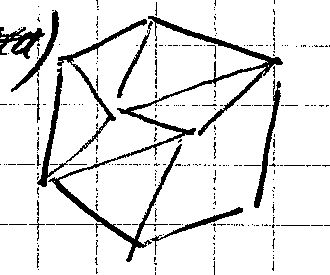
\includegraphics[width=\linewidth]{figures/gelfand-p001453-diagram-disk-original.png}
\par\smallskip{\footnotesize Оригинал рукописного рисунка: GELFAND-P001453\par}
\end{minipage}\hfill
\begin{minipage}[c]{0.48\linewidth}\centering
\resizebox{\linewidth}{!}{% Partial trace in crop-pixel coordinates. All visible gaps remain unjoined.
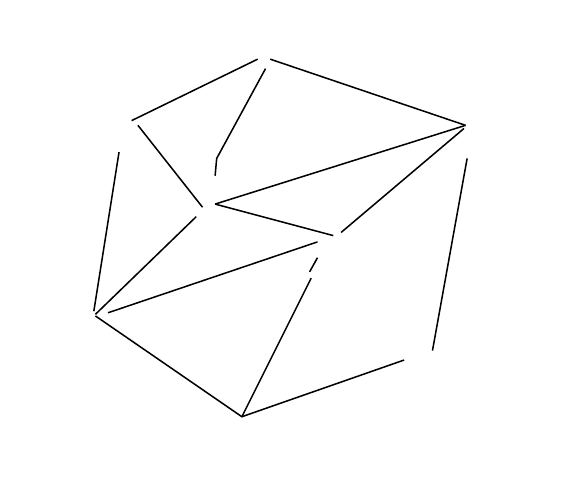
\begin{tikzpicture}[x=0.02cm,y=-0.02cm,line width=0.55pt]
\path[use as bounding box] (0,0) rectangle (330,275);
\draw (66,59)--(146,20);
\draw (154,20)--(278,62);
\draw (279,83)--(257,205);
\draw (239,211)--(136,247)--(43,183);
\draw (42,180)--(58,79);
\draw (70,62)--(111,114);
\draw (107,120)--(43,182);
\draw (119,112)--(194,132);
\draw (199,130)--(277,64);
\draw (119,112)--(278,62);
\draw (136,247)--(180,159);
\draw (184,146)--(179,155);
\draw (151,26)--(120,83)--(119,94);
\draw (51,181)--(184,136);
\end{tikzpicture}
}
\par\smallskip{\footnotesize Частичное воссоздание видимых штрихов; неясные соединения и подписи явно отмечены.\par}
\end{minipage}\par\medskip


(1) Надо док., что вершины можно так закрасить в 4 цвета
[\RussianUnclear{GELFAND-P001453}{line-one-cancellation}{зачёркнутый короткий фрагмент неразборчив}],
чтобы соседние вершины были раскрашены в разные цвета.

[Мелкая приписка:] (это двойств. задача к раскр. граней; поэтому
\RussianUnclear{GELFAND-P001453}{parenthetical-tail}{другая только?; другие только?}

(2) Мн-во конфигур. наз. \underline{неизбежным}, если в каждой триангул.
одна из них встречается.

(3) Конфиг. наз. \underline{приводимой}, если она не может входить в
триангуляцию сферы, не раскрашиваемую в 4 цвета и
имеющую среди таких триангуляций наименьшее число вершин.

\underline{Привод. триангуляция $K$:}
[зачёркнуто: \RussianUnclear{GELFAND-P001453}{reducibility-cancelled-if}{если?}; вписано сверху: «пусть»]
есть триан. $T\supset K$ и известно,
что $\forall$ конфигур. [\RussianUnclear{GELFAND-P001453}{reducibility-cancelled-word}{зачёркнутое слово неразборчиво}]
с меньшим числом вершин (чем $T$)
раскрашивается в 4 цвета; тогда и $T$ тоже раскрашивается.

Индукция по числу вершин $N$.

\underline{Пусть для $N-1$ вершин уже доказано.}

Конфиг. [зачёркнуто: \RussianUnclear{GELFAND-P001453}{induction-cancelled-word}{это?}] $K$ наз. \underline{приводимой}, если
[вписано сверху: «из»] её присутствия в $T$ с
$|T|=N$ следует, что $T$ раскрашивается.

[Зачёркнуто: «Пример.»]

Основная идея — соединение определений (2) и (3).

[Зачёркнуто: «Нужно»; вписано сверху: «Достаточно»]
построить неизбежный набор приводимых конфигураций.

(4) \underline{Пример.}

\begin{center}
\begin{tikzpicture}[x=1cm,y=1cm]
\draw (0,0)--(.8,1.3)--(1.8,.1)--cycle;
\draw (.8,.55)--(0,0) (.8,.55)--(.8,1.3) (.8,.55)--(1.8,.1);
\fill (0,0) circle (2pt);
\fill (.8,1.3) circle (2pt);
\fill (1.8,.1) circle (2pt);
\fill (.8,.55) circle (2pt);
\node[anchor=west] at (2.2,.65) {— приводимая конфигурация.};
\end{tikzpicture}
\end{center}

\begin{center}
\begin{tikzpicture}[x=1cm,y=1cm]
\draw (0,0)--(.8,1.3)--(1.8,.1)--cycle;
\draw (.8,.55)--(0,0) (.8,.55)--(.8,1.3) (.8,.55)--(1.8,.1);
\draw (-.65,.8)--(-.2,.4) (.4,1.9)--(.7,1.4)
      (1.6,1.8)--(1.2,1.35) (2.4,1.15)--(1.9,.55)
      (-.3,-.65)--(-.25,-.45) (.85,-.6)--(.95,-.2)
      (1.4,-.65)--(1.4,-.25) (2.25,-.5)--(2.1,-.05);
\draw[->] (2.9,.65)--(4.6,.65);
\draw (6.1,.1)--(6.9,1.2)--(7.55,.1)--cycle;
\draw (5.35,1.35)--(5.95,.55) (6.05,1.85)--(6.6,1.05)
      (7.8,1.85)--(7.55,1.2) (8.45,1.3)--(7.8,.65)
      (8.65,.3)--(7.95,-.2) (6.9,-.85)--(7.1,-.25)
      (5.85,-.9)--(6.25,-.4) (5.2,-.6)--(5.55,-.3);
\node[align=center] at (7,-1.45) {тоже\\триангуляция};
\end{tikzpicture}
\end{center}



\RussianSourceFrame{GELFAND-P001454}{unlabelled}
\underline{И.М.Г.} Всё надо придумывать на простейших примерах.
(И. Бернштейн этому науч. от И.М.Г.)

Теор. сферич. ф-й И.М.Г. придумал всю на ф-ле
\begin{equation*}
\cos(\alpha+\beta)+\cos(\alpha-\beta)=2\cos\alpha\cdot\cos\beta.
\end{equation*}
На $\mathbb R$ надо рассм. группу, порожденную паралл. переносами и
отражениями.

[Над следующим заголовком зачёркнуто: \RussianUnclear{GELFAND-P001454}{cancelled-theorem-heading}{Утв.?}]

(5) \underline{Теорема}
\begin{center}
\begin{tikzpicture}[x=1cm,y=1cm]
\draw (0,0)--(.25,1.4)--(1.7,1.45)--(1.5,.1)--cycle;
\draw (0,0)--(.88,.73)--(1.7,1.45);
\draw (.25,1.4)--(.88,.73)--(1.5,.1);
\fill (0,0) circle (2pt);
\fill (.25,1.4) circle (2pt);
\fill (1.7,1.45) circle (2pt);
\fill (1.5,.1) circle (2pt);
\fill (.88,.73) circle (2pt);
\node[anchor=west] at (2.5,.75) {приводима};
\end{tikzpicture}
\end{center}

(Кемпе; $\sim 100$ лет назад)

Заменим на

(6)
\begin{center}
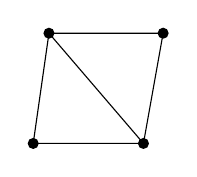
\begin{tikzpicture}[x=1cm,y=1cm]
\draw (0,0)--(.2,1.4)--(1.65,1.4)--(1.4,0)--cycle;
\draw (.2,1.4)--(1.4,0);
\fill (0,0) circle (2pt);
\fill (.2,1.4) circle (2pt);
\fill (1.65,1.4) circle (2pt);
\fill (1.4,0) circle (2pt);
\end{tikzpicture}
\end{center}
и раскрасим получившуюся триангуляцию.

(*) Если среди 4-х есть одинаковые, то центр раскр. в свободную.
\begin{center}
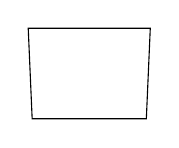
\begin{tikzpicture}[x=1cm,y=1cm]
\draw (0,0)--(-.05,1.15)--(1.5,1.15)--(1.45,0)--cycle;
\end{tikzpicture}
\end{center}

остаётся рассм. случай

(7)
\begin{center}
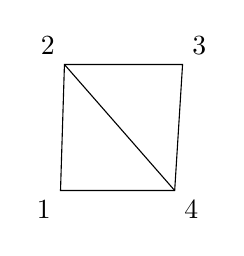
\begin{tikzpicture}[x=1cm,y=1cm]
\draw (0,0)--(.05,1.6)--(1.55,1.6)--(1.45,0)--cycle;
\draw (.05,1.6)--(1.45,0);
\node[below left] at (0,0) {$1$};
\node[above left] at (.05,1.6) {$2$};
\node[above right] at (1.55,1.6) {$3$};
\node[below right] at (1.45,0) {$4$};
\end{tikzpicture}
\end{center}

Рассм. подмн-во $K$, сост. из вершин, раскр. в 1 и 3
и рёбер
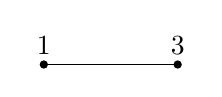
\begin{tikzpicture}[baseline=0pt,x=1cm,y=1cm]
\draw (0,0)--(1.7,0);
\fill (0,0) circle (1.5pt);
\fill (1.7,0) circle (1.5pt);
\node[above] at (0,0) {$1$};
\node[above] at (1.7,0) {$3$};
\end{tikzpicture}

(8) 1 может а) соединяться с 3 в $K$

или б) не соединяться.

Случай б): в этой связной компоненте вершины 1
меняем 1 и 3 местами и сводим к пред. случаю (*).

(9)
\RussianSourceFigure{GELFAND-P001454}{diagram-path}{Квадрат с диагональю из верхней левой вершины к нижней правой; у углов подписи: слева внизу 1, слева вверху 2, справа вверху 3, справа внизу 4. Снаружи снизу и справа проходит линия со сплошной начальной частью и отдельными штрихами продолжения; у её нижних изломов видны 3, 1 и исправленная цифра, похожая на 3. Точный вид последней подписи и примыкания штрихового продолжения проверить по оригиналу.}

\par\medskip\noindent
\begin{minipage}[c]{0.48\linewidth}\centering
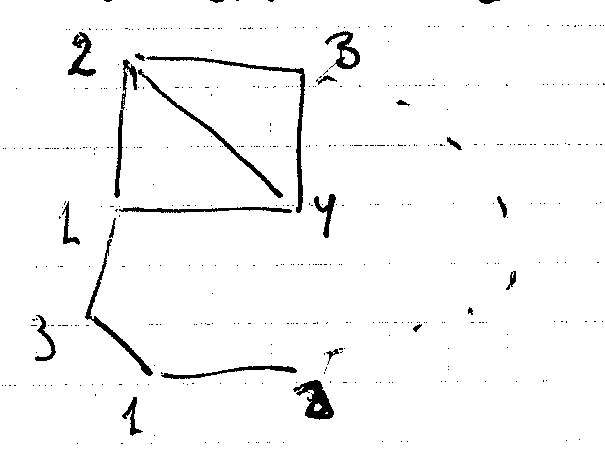
\includegraphics[width=\linewidth]{figures/gelfand-p001454-diagram-path-original.png}
\par\smallskip{\footnotesize Оригинал рукописного рисунка: GELFAND-P001454\par}
\end{minipage}\hfill
\begin{minipage}[c]{0.48\linewidth}\centering
\resizebox{\linewidth}{!}{% Partial source-stroke trace. The right-hand continuation stays separate.
% The bracketed bottom digit is an uncertainty marker, not a new decipherment.
\begin{tikzpicture}[x=0.01cm,y=-0.01cm,line width=0.55pt]
\path[use as bounding box] (0,0) rectangle (605,460);
\draw (118,194)--(123,68);
\draw (136,58)--(302,71)--(300,210);
\draw (117,210)--(291,210);
\draw (135,75)--(281,195);
\draw (113,242)--(87,316)--(148,373);
\draw (163,376)..controls(207,379)and(247,362)..(295,371);
\draw (398,104)--(407,105);
\draw (447,139)--(461,150);
\draw (500,198)--(506,214);
\draw (514,272)--(511,286);
\draw (470,307)--(473,314);
\draw (415,328)--(423,321);
\node at (76,55) {$2$};\node at (345,46) {$3$};
\node at (67,230) {$1$};\node at (325,216) {$4$};
\node at (45,340) {$3$};\node at (132,418) {$1$};
\node at (330,410) {$[3/8\,?]$};
\end{tikzpicture}
}
\par\smallskip{\footnotesize Частичное воссоздание видимых штрихов; неясные соединения и подписи явно отмечены.\par}
\end{minipage}\par\medskip


[Справа от рисунка:]

Пусть случай 8а).

Тогда не сущ. пути из 2 в 4
с [зачёркнуто: \RussianUnclear{GELFAND-P001454}{cancelled-before-two}{зачёркнутый фрагмент неразборчив}] 2 и 4.

\RussianSourceFigure{GELFAND-P001454}{diagram-excluded-edge}{Два маленьких рисунка: квадрат с диагональю и отдельно наклонное ребро. На диагонали и на отдельном ребре одинаковый петлеобразный знак исключения. Подпись справа: «— это ребро не считаем». Точный рисунок петлеобразной пометы проверить по оригиналу.}

\par\medskip\noindent
\begin{minipage}[c]{0.48\linewidth}\centering
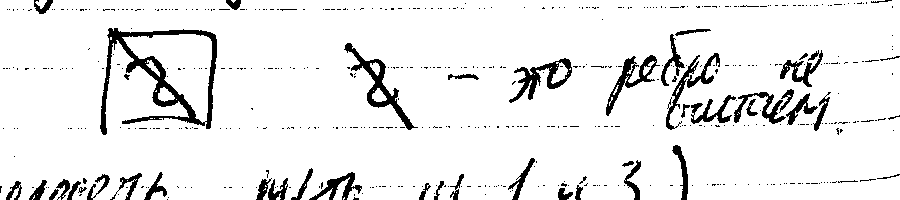
\includegraphics[width=\linewidth]{figures/gelfand-p001454-diagram-excluded-edge-original.png}
\par\smallskip{\footnotesize Оригинал рукописного рисунка: GELFAND-P001454\par}
\end{minipage}\hfill
\begin{minipage}[c]{0.48\linewidth}\centering
\resizebox{\linewidth}{!}{\def\ExcludedEdgeCaption{Это ребро не считаем.}
% Literal two-loop edge annotation; it adds no graph vertex.
\begin{tikzpicture}[x=0.01cm,y=-0.01cm,line width=0.55pt]
\path[use as bounding box] (0,0) rectangle (900,175);
\draw (104,130)--(110,33)--(214,32)--(210,126);
\draw (121,124)..controls(160,111)and(187,114)..(201,122);
\draw (114,36)--(197,118);
\draw (129,73)..controls(145,48)and(161,60)..(160,76)
 ..controls(158,89)and(140,100)..(155,104)
 ..controls(172,108)and(180,97)..(178,91);
\draw (346,47)--(410,127);
\draw (346,77)..controls(366,49)and(383,64)..(381,78)
 ..controls(379,94)and(357,109)..(372,114)
 ..controls(389,118)and(402,105)..(399,97);
\node[anchor=west,text width=3.7cm,align=left] at (455,80) {\ExcludedEdgeCaption};
\end{tikzpicture}
}
\par\smallskip{\footnotesize Частичное воссоздание видимых штрихов; неясные соединения и подписи явно отмечены.\par}
\end{minipage}\par\medskip


(т.к. не может пересечь путь из 1 и 3)

и дальше опять сводим к 8б).


